% douglas_peucker.tex
% Requires in main preamble:
% \usepackage{tikz}

% Original polyline path - for plot coordinates, NO commas between coordinates
\def\RawPath{
	(0,0) (1,1) (2,2) (2,3) (3,4) (4,5) (4,6) (5,7) (5,8) (6,9)
	(7,10) (7,11) (8,12) (8,13) (9,14) (9,15) (10,16) (11,17) (12,18) (13,18)
	(14,19) (15,19) (16,19) (17,20) (18,20) (19,20) (20,21) (21,21) (22,21) (23,22)
	(24,22) (25,22) (26,22) (27,22) (28,22) (29,23) (30,23) (31,23) (32,23) (33,23)
	(34,24) (35,24) (36,24) (37,25) (38,25) (39,25) (40,25) (41,25) (42,25) (43,25)
	(44,25) (45,25) (46,25) (47,26) (48,26) (49,26) (50,26) (51,26) (52,26) (53,26)
	(54,26) (55,26) (56,26) (57,26) (58,26) (59,26) (60,27) (61,27) (62,27) (63,27)
	(64,27) (65,27) (66,27) (67,27) (68,27) (69,27) (70,27) (71,26) (72,26) (73,26)
	(74,27) (75,26) (76,26) (77,26) (78,26) (79,26) (80,26) (81,26) (82,26) (83,26)
	(84,26) (85,26) (86,26) (87,26) (88,26) (89,26) (90,26) (91,26) (92,26) (93,26)
	(94,26) (95,26) (96,25) (97,25) (98,25) (99,26)
}

% Original polyline list - for foreach, coordinates must be wrapped in braces
\def\RawList{
	{(0,0)},{(1,1)},{(2,2)},{(2,3)},{(3,4)},{(4,5)},{(4,6)},{(5,7)},{(5,8)},{(6,9)},
	{(7,10)},{(7,11)},{(8,12)},{(8,13)},{(9,14)},{(9,15)},{(10,16)},{(11,17)},{(12,18)},{(13,18)},
	{(14,19)},{(15,19)},{(16,19)},{(17,20)},{(18,20)},{(19,20)},{(20,21)},{(21,21)},{(22,21)},{(23,22)},
	{(24,22)},{(25,22)},{(26,22)},{(27,22)},{(28,22)},{(29,23)},{(30,23)},{(31,23)},{(32,23)},{(33,23)},
	{(34,24)},{(35,24)},{(36,24)},{(37,25)},{(38,25)},{(39,25)},{(40,25)},{(41,25)},{(42,25)},{(43,25)},
	{(44,25)},{(45,25)},{(46,25)},{(47,26)},{(48,26)},{(49,26)},{(50,26)},{(51,26)},{(52,26)},{(53,26)},
	{(54,26)},{(55,26)},{(56,26)},{(57,26)},{(58,26)},{(59,26)},{(60,27)},{(61,27)},{(62,27)},{(63,27)},
	{(64,27)},{(65,27)},{(66,27)},{(67,27)},{(68,27)},{(69,27)},{(70,27)},{(71,26)},{(72,26)},{(73,26)},
	{(74,27)},{(75,26)},{(76,26)},{(77,26)},{(78,26)},{(79,26)},{(80,26)},{(81,26)},{(82,26)},{(83,26)},
	{(84,26)},{(85,26)},{(86,26)},{(87,26)},{(88,26)},{(89,26)},{(90,26)},{(91,26)},{(92,26)},{(93,26)},
	{(94,26)},{(95,26)},{(96,25)},{(97,25)},{(98,25)},{(99,26)}
}

% Douglas-Peucker result
\def\DpPath{
	(0,0) (12,18) (23,22) (60,27) (99,26)
}

\def\DpList{
	{(0,0)},{(12,18)},{(23,22)},{(60,27)},{(99,26)}
}

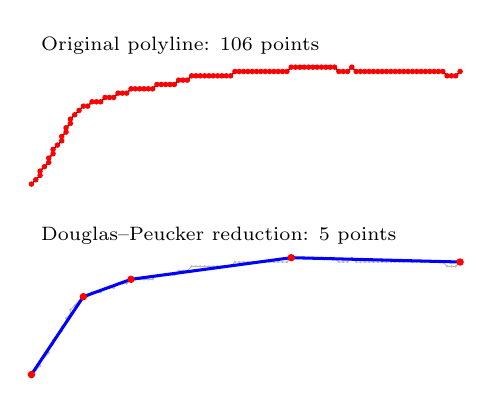
\begin{tikzpicture}[
	x=0.055cm,
	y=0.055cm,
	line cap=round,
	line join=round
	]
	
	% =========================================================
	% Original polyline
	% =========================================================
	\begin{scope}[shift={(0,38)}]
		\node[anchor=west, font=\scriptsize] at (0,32) {Original polyline: 106 points};
		
		\draw[black, line width=0.5pt] plot coordinates {\RawPath};
		
		\foreach \p in \RawList {
			\fill[red] \p circle (1.0pt);
		}
	\end{scope}
	
	% =========================================================
	% Douglas-Peucker simplified polyline
	% =========================================================
	\begin{scope}[shift={(0,-6)}]
		\node[anchor=west, font=\scriptsize] at (0,32) {Douglas--Peucker reduction: 5 points};
		
		% Original in background
		\draw[gray!55, line width=0.35pt] plot coordinates {\RawPath};
		
		\foreach \p in \RawList {
			\fill[gray!55] \p circle (0.45pt);
		}
		
		% Simplified result
		\draw[blue, line width=1.1pt] plot coordinates {\DpPath};
		
		\foreach \p in \DpList {
			\fill[red] \p circle (1.35pt);
		}
	\end{scope}
	
\end{tikzpicture}